\begin{adjustwidth*}{}{-2.25in}
\textbf{{\large Exercises}}
\setlength{\columnsep}{25pt}
\begin{multicols*}{2}
\noindent Terms and Concepts \small
\begin{enumerate}[1)]
\item Explain in  your own words what the second derivative ``means.''
\item If $f(x)$ describes a position function, then $f'(x)$ describes what kind of function? What kind of function is $f''(x)$?
\item Let $f(x)$ be a function measured in pounds, where $x$ is measured in feet. What are the units of $f''(x)$?
\item Explain in your own words how to find the third derivative of a function $f(x)$.
\end{enumerate} 

\noindent {\normalsize Problems} \small

%\noindent {\bf In exercises 5--8, a graph of a function is given. Using the graph, sketch $f'(x)$.}

\begin{enumerate}[1),resume]
\item Suppose that $y = f(x)$ is a differentiable function for which the following information is known:  $f(2) = -3$, $f'(2) = 1.5$, $f''(2) = -0.25$.
\ba
	\item Is $f$ increasing or decreasing at $x = 2$?  Is $f$ concave up or concave down at $x = 2$?
	\item Do you expect $f(2.1)$ to be greater than $-3$, equal to $-3$, or less than $-3$?  Why?
	\item Do you expect $f'(2.1)$ to be greater than $1.5$, equal to $1.5$, or less than $1.5$?  Why?
	\item Sketch a graph of $y = f(x)$ near $(2,f(2))$ and include a graph of the tangent line.  
\ea

\item For a certain function $y = g(x)$, its derivative is given by the function pictured below.
\begin{center}
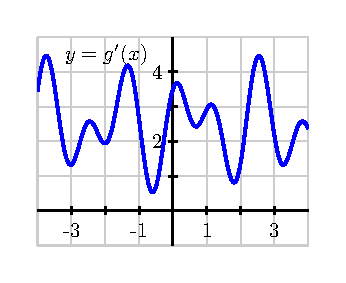
\includegraphics[scale=.75]{figures/1_6_Ez2.eps}
\end{center}
\ba
	\item What is the approximate slope of the tangent line to $y = g(x)$ at the point $(2,g(2))$?
	\item How many real number solutions can there be to the equation $g(x) = 0$?  Justify your conclusion fully and carefully by explaining what you know about how the graph of $g$ must behave based on the given graph of $g'$.
	\item On the interval $-3 < x < 3$, how many times does the concavity of $g$ change?  Why?
	\item Use the provided graph to estimate the value of $g''(2)$.
\ea

\item For each prompt that follows, sketch a possible graph of a function on the interval $-3 < x < 3$ that satisfies the stated properties.
\ba
	\item $y = f(x)$ such that $f$ is increasing on $-3 < x < 3$, $f$ is concave up on $-3 < x < 0$, and $f$ is concave down on $0 < x < 3$.
	\item $y = g(x)$ such that $g$ is increasing on $-3 < x < 3$, $g$ is concave down on $-3 < x < 0$, and $g$ is concave up on $0 < x < 3$.
	\item $y = h(x)$ such that $h$ is decreasing on $-3 < x < 3$, $h$ is concave up on $-3 < x < -1$, neither concave up nor concave down on $-1 < x < 1$, and $h$ is concave down on $1 < x < 3$.
	\item $y = p(x)$ such that $p$ is decreasing and concave down on $-3 < x < 0$ and $p$ is increasing and concave down on $0 < x < 3$.
\ea

\item A bungee jumper's height $h$ (in feet ) at time $t$ (in seconds) is given in the table below.
\ba
	\item Use the given data to estimate $h'(4.5)$, $h'(5)$, and $h'(5.5)$.  At which of these times is the bungee jumper rising most rapidly?
	\item Use the given data and your work in (a) to estimate $h''(5)$.
	\item What physical property of the bungee jumper does the value of $h''(5)$ measure?  What are its units?
	\item Based on the data, on what approximate time intervals is the function $y = h(t)$ concave down?  What is happening to the velocity of the bungee jumper on these time intervals?
\ea

\begin{center}
\begin{tabular}{ccc}
\begin{tabular}{| l | l |} \hline
$t$ & $h(t)$ \\ \hline \hline
$0.0$ & $200$ \\ \hline
$0.5$ & $184.2$ \\ \hline
$1.0$ & $159.9$ \\ \hline
$1.5$ & $131.9$ \\ \hline
$2.0$ & $104.7$ \\ \hline
$2.5$ & $81.8$ \\ \hline
$3.0$ & $65.5$ \\ \hline
$3.5$ & $56.8$ \\ \hline
$4.0$ & $55.5$ \\ \hline
$4.5$ & $60.4$ \\ \hline
$5.0$ & $69.8$ \\ \hline
\end{tabular}
& &
\begin{tabular}{| l | l |} \hline
$t$ & $h(t)$ \\ \hline \hline
$5.5$ & $81.6$ \\ \hline
$6.0$ & $93.7$ \\ \hline
$6.5$ & $104.4$ \\ \hline
$7.0$ & $112.6$ \\ \hline
$7.5$ & $117.7$ \\ \hline
$8.0$ & $119.4$ \\ \hline
$8.5$ & $118.2$ \\ \hline
$9.0$ & $114.8$ \\ \hline
$9.5$ & $110.0$ \\ \hline
$10.0$ & $104.7$ \\ \hline
\end{tabular}
\end{tabular}
\end{center}

\end{enumerate}

%------------------------------------------
% END OF EXERCISES ON FIRST PAGE
%------------------------------------------
\end{multicols*}
\end{adjustwidth*}

\afterexercises